\section{Advanced Operating Techniques}
\label{section:advanced_operating}

\subsection*{FM Transmission Distortion}
FM transmission distortion on voice peaks can occur when the input audio signal is too loud, causing over-modulation. This results in distorted audio at the receiving end. To avoid this, ensure that your microphone gain is properly adjusted and avoid speaking too loudly into the microphone. Over-modulation can also be caused by excessive transmit power, but this is less common in modern equipment.


\subsection*{Digital Repeater Talkgroups}
To join a digital repeater's talkgroup, you need to program your radio with the group's ID or code. Talkgroups allow multiple users to communicate on the same digital repeater without interfering with each other. Each talkgroup has a unique identifier, and your radio must be configured to use the correct ID to access the group. This system is commonly used in DMR (Digital Mobile Radio) networks.

\subsection*{Frequency Interference Management}
\begin{wrapfigure}{r}{0.35\textwidth}
    \centering
    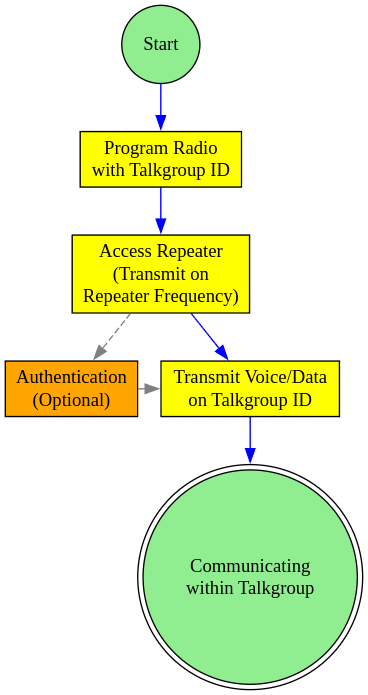
\includegraphics[width=0.3\textwidth]{tech/organized/chapter_2/images/talkgroup.png}
    \caption{Joining a Digital Repeater Talkgroup}
    \label{fig:talkgroup}
    % Diagram showing the process of joining a digital repeater talkgroup. The diagram should include steps like programming the radio with the group ID, accessing the repeater, and communicating within the talkgroup.
\end{wrapfigure}

When two stations transmit on the same frequency and interfere with each other, they should negotiate continued use of the frequency. This is a common practice in amateur radio to ensure fair and efficient use of the spectrum. The Q signal \textbf{QRM} indicates that you are receiving interference from other stations, while \textbf{QSY} indicates that you are changing frequency to avoid interference.


\begin{table}[h!]
    \centering
    \caption{Common Q Signals and Their Detailed Meanings}
    \begin{tabular}{|l|p{5.5cm}|p{5.5cm}|}
        \hline
        \textbf{Code} & \textbf{When Asked as Question} & \textbf{When Used as Statement} \\
        \hline
        QRA & What ship or coast station is that? & This is \_\_\_\_. \\
        \hline
        QRB & What is your distance? & My distance is \_\_\_\_ kilometers/miles. \\
        \hline
        QRC & What is your true bearing? & My true bearing is \_\_\_\_ degrees. \\
        \hline
        QRD & Where are you bound for? & I am bound for \_\_\_\_. \\
        \hline
        QRF & Where are you bound from? & I am bound from \_\_\_\_. \\
        \hline
        QRG & What line do you belong to? & I belong to the \_\_\_\_ Line. \\
        \hline
        QRH & What is your wavelength in meters? & My wavelength is \_\_\_\_ meters. \\
        \hline
        QRJ & How many words have you to send? & I have \_\_\_\_ words to send. \\
        \hline
        QRK & How do you receive me? & I receive you: 1 (unreadable) to 5 (perfect). \\
        \hline
        QRL & Are you busy? & I am busy. Please do not interfere. \\
        \hline
        QRM & Are you being interfered with? & I am being interfered with. \\
        \hline
        QRN & Are the atmospherics strong? & Atmospheric noise is very strong. \\
        \hline
    \end{tabular}
    \label{tab:q_signals}
\end{table}

Q signals can be used either as questions (by adding a question mark) or as statements. These signals are particularly useful because they:
\begin{itemize}
    \item Are internationally recognized
    \item Overcome language barriers
    \item Provide quick, standardized communication
    \item Work well in poor signal conditions
\end{itemize}

\subsection*{Using Q Signals}
Q signals are a standardized set of three-letter codes, all beginning with 'Q', that facilitate efficient communication, especially in poor conditions or across language barriers. These signals can be used in two ways:

\begin{itemize}
    \item As a question by adding a question mark
    \item As a statement by providing the information
\end{itemize}

Common usage examples:
\begin{itemize}
    \item \textbf{Location Exchange}:
        \begin{itemize}
            \item Question: "QTH?"
            \item Response: "QTH Atlanta, Georgia"
            \item Meaning: "What is your location?" / "My location is Atlanta, Georgia"
        \end{itemize}
    \item \textbf{Signal Report}:
        \begin{itemize}
            \item Question: "QRK?"
            \item Response: "QRK 4"
            \item Meaning: "How do you receive me?" / "I receive you well (4 out of 5)"
        \end{itemize}
    \item \textbf{Interference Check}:
        \begin{itemize}
            \item Statement: "QRM" or "QRM?"
            \item Response: "QSY 7.255"
            \item Meaning: "I am experiencing interference" / "Let's change frequency to 7.255 MHz"
        \end{itemize}
    \item \textbf{Frequency Usage}:
        \begin{itemize}
            \item Question: "QRL?"
            \item Response: "QRL" or "YES QRL"
            \item Meaning: "Is this frequency in use?" / "Yes, this frequency is in use"
        \end{itemize}
\end{itemize}

In practice, Q signals are often combined with standard voice communications. For example:
\begin{itemize}
    \item "QTH is Atlanta, name is John"
    \item "Getting QRM from nearby station, QSY up 5"
    \item "QRK 5, you are perfectly readable here"
\end{itemize}

\subsection*{Questions}
\begin{tcolorbox}[colback=gray!10!white,colframe=black!75!black,title={T2B05}]
    What would cause your FM transmission audio to be distorted on voice peaks?
    \begin{enumerate}[label=\Alph*),noitemsep]
        \item Your repeater offset is inverted
        \item You need to talk louder
        \item \textbf{You are talking too loudly}
        \item Your transmit power is too high
    \end{enumerate}
\end{tcolorbox}
Distortion on voice peaks in FM transmission is typically caused by over-modulation, which occurs when the input audio signal is too loud. This can be avoided by adjusting the microphone gain and speaking at a normal volume. Excessive transmit power is less likely to cause distortion in modern equipment.

%memory_trick T2B05

\begin{tcolorbox}[colback=gray!10!white,colframe=black!75!black,title={T2B06}]
    What type of signaling uses pairs of audio tones?
    \begin{enumerate}[label=\Alph*),noitemsep]
        \item \textbf{DTMF}
        \item CTCSS
        \item GPRS
        \item D-STAR
    \end{enumerate}
\end{tcolorbox}
DTMF (Dual-Tone Multi-Frequency) signaling uses pairs of audio tones to represent numbers, letters, or special characters. This method is widely used in amateur radio for remote control and automated systems.

%memory_trick T2B06

\begin{tcolorbox}[colback=gray!10!white,colframe=black!75!black,title={T2B07}]
    How can you join a digital repeater’s “talkgroup”?
    \begin{enumerate}[label=\Alph*),noitemsep]
        \item Register your radio with the local FCC office
        \item Join the repeater owner’s club
        \item \textbf{Program your radio with the group’s ID or code}
        \item Sign your call after the courtesy tone
    \end{enumerate}
\end{tcolorbox}
To join a digital repeater's talkgroup, you need to program your radio with the group's ID or code. This allows you to communicate within the designated group without interfering with other users on the same repeater.

%memory_trick T2B07

\begin{tcolorbox}[colback=gray!10!white,colframe=black!75!black,title={T2B08}]
    Which of the following applies when two stations transmitting on the same frequency interfere with each other?
    \begin{enumerate}[label=\Alph*),noitemsep]
        \item \textbf{The stations should negotiate continued use of the frequency}
        \item Both stations should choose another frequency to avoid conflict
        \item Interference is inevitable, so no action is required
        \item Use subaudible tones so both stations can share the frequency
    \end{enumerate}
\end{tcolorbox}
When two stations interfere on the same frequency, they should negotiate to determine who will continue using the frequency. This is a common practice in amateur radio to ensure fair use of the spectrum.

%memory_trick T2B08

\begin{tcolorbox}[colback=gray!10!white,colframe=black!75!black,title={T2B09}]
    Why are simplex channels designated in the VHF/UHF band plans?
    \begin{enumerate}[label=\Alph*),noitemsep]
        \item \textbf{So stations within range of each other can communicate without tying up a repeater}
        \item For contest operation
        \item For working DX only
        \item So stations with simple transmitters can access the repeater without automated offset
    \end{enumerate}
\end{tcolorbox}
Simplex channels are designated in the VHF/UHF band plans to allow stations within range of each other to communicate directly without using a repeater. This is useful for local communication and reduces the load on repeater systems.

%memory_trick T2B09

\begin{tcolorbox}[colback=gray!10!white,colframe=black!75!black,title={T2B10}]
    Which Q signal indicates that you are receiving interference from other stations?
    \begin{enumerate}[label=\Alph*),noitemsep]
        \item \textbf{QRM}
        \item QRN
        \item QTH
        \item QSB
    \end{enumerate}
\end{tcolorbox}
The Q signal \textbf{QRM} indicates that you are receiving interference from other stations. This is a common issue in crowded frequency bands, and operators may need to change frequencies to avoid the interference.

%memory_trick T2B10

\begin{tcolorbox}[colback=gray!10!white,colframe=black!75!black,title={T2B11}]
    Which Q signal indicates that you are changing frequency?
    \begin{enumerate}[label=\Alph*),noitemsep]
        \item QRU
        \item \textbf{QSY}
        \item QSL
        \item QRZ
    \end{enumerate}
\end{tcolorbox}
The Q signal \textbf{QSY} indicates that you are changing frequency. This is often used to avoid interference or to move to a clearer frequency for communication.

%memory_trick T2B11

\begin{tcolorbox}[colback=gray!10!white,colframe=black!75!black,title={T2B12}]
    What is the purpose of the color code used on DMR repeater systems?
    \begin{enumerate}[label=\Alph*),noitemsep]
        \item \textbf{Must match the repeater color code for access}
        \item Defines the frequency pair to use
        \item Identifies the codec used
        \item Defines the minimum signal level required for access
    \end{enumerate}
\end{tcolorbox}
The color code in DMR repeater systems is used to ensure that your radio matches the repeater's color code for access. This helps prevent unauthorized access and ensures compatibility between radios and repeaters.

%memory_trick T2B12

\subsection*{Summary}
This section covered advanced operating techniques in amateur radio, including:
\begin{itemize}
    \item \textbf{FM Transmission Distortion}: Caused by over-modulation due to excessive audio input. Adjust microphone gain to avoid distortion.
    \item \textbf{DTMF Signaling}: Uses pairs of audio tones for remote control and automated functions in amateur radio.
    \item \textbf{Digital Repeater Talkgroups}: Join by programming your radio with the group's ID or code to communicate within a specific group.
    \item \textbf{Frequency Interference Management}: Use Q signals like QRM and QSY to manage and avoid interference on shared frequencies.
\end{itemize}
